\documentclass[reqno]{amsart}
\usepackage{fancyhdr}
\usepackage{amsmath}
\usepackage{amssymb}
\usepackage{pifont}
\usepackage{booktabs}
\usepackage{subcaption}
\usepackage{graphicx}
\usepackage{verbatim}
\usepackage{hyperref}


\pagestyle{fancy}
\chead{10/24/21}
\rhead{Jackson Dougherty}
\renewcommand{\headrulewidth}{0.4pt}
\renewcommand{\footrulewidth}{0.4pt}

\hypersetup{
    colorlinks=true,     
    urlcolor=blue,
    }

\begin{document}
\section*{Riddler 10-24-21}
\section*{Jackson Dougherty}

\section{Riddler Classic}

\subsection*{Problem}

Suppose you have an equilateral triangle. You pick three random points, one along each of its three edges, uniformly along the length of each edge — that is, each point along each edge has the same probability of being selected.

With those three randomly selected points, you can form a new triangle inside the original one. What is the probability that the center of the larger triangle also lies inside the smaller one?

\subsection*{Solution}

Preview: for an analytic solution, we embed the equilateral triangle in the Cartesian plane. Then, the randomly selected points can each be represented by a single parameter. The inner triangle will also be represented by equations in the plane. The condition regarding the center of the larger triangle will then become a set of inequalities in the three parameters. We can measure the volume of the space where these inequalities are satisfied, and this volume will represent our probability, with appropriate scaling of the parameters. 

We embed the equilateral triangle with its base along the x-axis, and with side length 2. Then, its vertices are at $(0,0)$, $(0,2)$, and $(1, \sqrt{3})$. The center is then located at $(x_c, y_c) =(1,\sqrt{3}/2)$. 

We will parametrize the sides using parameters $t_1, t_2, t_3$ that range from $0$ to $1$. We will move along the triangle counter-clockwise in these parameters. With this range, $2t_i$ then represents the distance traveled along the $i$th side. The coordinates of the random points are notated $(x_i, y_i)$ for $i=1,2,3$. 

\begin{align*}
x_1 &= 2t_1 \\
y_1 &= 0 \\
x_2 &=  2 - t_2 \\
y_2 &= t_2 \sqrt{3} \\
x_3 &= 1-t_3 \\
y_3 &= \sqrt{3}(1-t_3)
\end{align*}

Now we can write the equation of the lines that form the inner triangle in terms of the coordinates of the selected points. 

For the line joining the base and the right side of the triangle, we can write the following equation,
\begin{align*}
y-y_1 &= \frac{y_2-y_1}{x_2-x_1} (x-x_1) \\
y &= \frac{t_2 \sqrt{3}}{2- t_2 - 2t_1} (x-2t_1).
\end{align*}

Then, for the center to be contained in the inner triangle, it is necessary that its coordinates satisfy an inequality involving this equation,
\begin{align*}
\sqrt{3}/2 &\geq \frac{t_2 \sqrt{3}}{2-t_2-2t_1} (1 - 2t_1)
\end{align*} 
which we may rearrange as 
\begin{align*}
4t_1 t_2 -3t_2-2t_1+2\geq 0,
\end{align*}
in the case where $x_2-x_1>0$. In the case where $x_2-x_1<0$, the leg joining sides one and two of the inner triangle has negative slope, and lies completely to the right of $x_2>x_c$, implying that this leg will not leave the center outside the inner triangle. 

We can write the same sort of equation for the upper leg of the inner triangle, joining the right and left sides of the outer triangle, 
\begin{align*}
y- y_3 &= \frac{y_2-y_3}{x_2-x_3}(x-x_3) \\
y- \sqrt{3}(1-t_3) &= \frac{\sqrt{3}(t_2 - (1-t_3))}{(2-t_2)-(1-t_3)}(x-(1-t_3)) \\
y/\sqrt{3}-1+t_3 & = \frac{t_2+t_3-1}{1+t_3-t_2}(x-1+t_3).
\end{align*}

As before, we can form an inequality that represents a necessary condition for the center to lie inside the inner triangle,
\begin{align*}
1/2-1+t_3 &\leq \frac{t_2+t_3-1}{1+t_3-t_2}(1-1+t_3),
\end{align*}
which we may simplify since $x_2-x_3>0$ as
\begin{align*}
(2t_3-1)(1+t_3-t_2) &\leq 2t_3(t_2+t_3-1) \\
2t_3-1+2t_3^2-t_3-2t_2 t_3+t_2 &\leq 2t_2 t_3 + 2t_3^2-2t_3 \\
-4t_2 t_3 + 3t_3+t_2-1&\leq 0.
\end{align*}

Finally, we can write an equation for left leg of the inner triangle, joining the left side and base of the outer triangle,
\begin{align*}
y-y_1 &= \frac{y_1-y_3}{x_1-x_3}(x-x_1) \\
y &= \frac{-\sqrt{3}(1-t_3)}{2t_1-(1-t_3)}(x-2t_1).
\end{align*}

Similar to the first case, if $x_1<x_3$, then this leg cannot cause the triangle to fail to contain the center. Therefore, we consider the case of $x_1>x_3$, giving the inequality,
\begin{align*}
\frac{\sqrt{3}}{2} &\geq \frac{-\sqrt{3}(1-t_3)}{2t_1-(1-t_3)}(1-2t_1) \\
2t_1-1+t_3&\geq 2(t_3-1)(1-2t_1) \\
0 &\geq t_3+2t_1-4t_1t_3-1
\end{align*} 

Summarizing, we have a series of inequalities relating pairs of the three parameters $t_1, t_2, t_3$,
\begin{align*}
&\begin{cases}
2-t_2 \leq 2t_1 \\
4t_1 t_2 -3t_2-2t_1+2\geq 0,\\
\end{cases} \\
&3t_3+t_2-4t_2 t_3-1\leq 0, \\
&\begin{cases}
2t_1 \leq 1-t_3 \\
t_3+2t_1-4t_1t_3-1 \leq 0.
\end{cases}
\end{align*}

We can rearrange to ease integration,
\begin{align*}
&\begin{cases}
t_2 \geq 2-2t_1 \\
t_2\geq \frac{2t_1-2}{4t_1-3},\\
\end{cases} \\
&t_2 \geq \frac{3t_3-1}{4t_3-1}, \\
&\begin{cases}
t_1 \leq (1-t_3)/2 \\
t_1 \leq \frac{t_3-1}{4t_3-2}.
\end{cases}
\end{align*}

It is interesting that the conditions are not more symmetrical, although this seems to be mostly an artifact of the particular parametrization chosen. The first and third conditions appear to be reflected across the point $(t_1, t_i) =(1/2, 1/2)$, which is plausible since increasing $t_1$ and increasing $t_i$ each have opposite meanings depending on $i=2,3$. Increasing $t_1$ means getting closer to the right edge, but farther from the left edge. 
On the other hand, increasing $t_2$ means getting farther to the base, and increasing $t_3$ means getting closer to the base. By contrast, the condition on the left and right edges becomes more symmetrical in the two parameters under the transformation $t_3 \rightarrow 1-t_3$. Figure $\ref{plot:inequalitySlices}$ shows the regions of parameter space that satisfy these inequalities.

The lack of symmetry is a likely indicator of an error. Comparing a numerical estimate given by this parametrization to the analytic result shows an underestimate by approximately 0.05. The error of the numerical method is bounded by the surface area of the set, implying an inherent error of less than $0.005$. The larger difference reinforces that an error has likely occurred in the preceding logic. 

By choosing a specific interior triangle, and applying a little more knowledge of the inherent geometry, i.e. forgoing a specific parametrization, we could produce an integral that reflects the specific cases where the center is contained in inner triangle. Consult \href{https://puzzlingthroughmed.com/tricky-triangles/}{Allen Gu's proof} for more details. 

\begin{figure}[h]
	\centering
	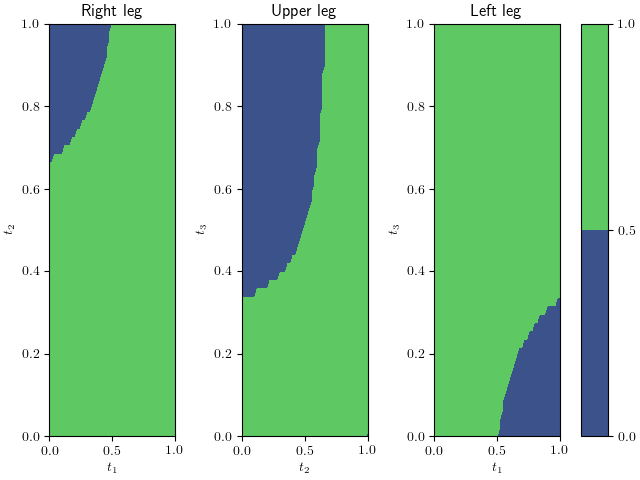
\includegraphics[scale = 0.75]{InequalitySlices.png}
	\caption{These plots visualize the parameter space where the inequalities are satisfied. The green areas are necessary for the center to be contained in the inner triangle.}
	\label{plot:inequalitySlices}
\end{figure}


\begin{comment}
We may also observe that the conditions on $t_2$ do not overlap. For $t_2 \in [0, 2/3]$, the condition on $t_3$ applies, whereas the condition on $t_1$ applies for $t_2 \in [2/3, 1]$. 


Now, we estimate the volume of the set where the inequalities are each satisfied,
\begin{align*}
V &= \int\int\int 1 \, dt_2\, dt_1 \, dt_3 \\
&= \int \int 1- \frac{2}{3}\frac{3t_3 -1}{4t_3-1} + \frac{1}{3}\frac{2t_1-2}{4t_1-3} dt_1 \, dt_3. \\
\end{align*}
The limits of integration for the $t_1$ integral can be given by the condition from $t_1$ and $t_3$. The lower limit is $0$, and the upper limit is $\min \left\lbrace 1, \frac{t_3-1}{4t_3-2}\right\rbrace$, ignoring the right branch of the rational function. Then, we may break the domain of $t_1$ into thirds and describe the behavior over each third,
\begin{align*}
\int \frac{1}{3} \int_0^{\frac{t_3-1}{4t_3-2}} 1-\frac{3t_3-1}{4t_3-1} \, dt_1 \, dt_3 \\
\end{align*}
\end{comment}

\end{document}